% !TEX root = ../notes_template.tex
\chapter{Econometric Models}\label{chp:Econometric_Models}

%\minitoc

%gls examples:
%\begin{itemize}
%	% \item \glsxtrshort{gcd};
%	\item \Gls{gcd}; \acrlong{gcd}; \acrshort{gcd}; \acrfull{gcd}
%\end{itemize}


%---- Section 1.1 ----%
\section{ECM and SEM}
\cite{NaiefEltony1995}\\
%\begin{multicols}{2}
	 \paragraph{}{This paper tests two models for energy demand projection on Kuwait data and forecast the future energy demand in Kuwait. The long-run and short-run price and income elasticities were estimated. The root mean square percent error (RMSPE) and mean percent error (MPE) measured the deviation of the estimates from the observations. }
%\end{multicols}


%---- 1.1.1 Subsection 1 ----%
\subsection{Method 1: ECM}
\paragraph{}{
\textbf{Cointegration and Error-Correction Model (ECM)} takes into account the time-series characteristics of the data. It combines cointegration techniques and an error-correction model and has the advantages of
\begin{itemize}
	% \item \glsxtrshort{gcd};
	\item Being easy to distinguish between the short- and long- run response.
	\item Estimating the speed of adjustment toward the long-run values.
\end{itemize} 	
}

\paragraph{Three-step projection}{
	\begin{enumerate}
		\item \textbf{Examine the time-series effect. }\\
		To test if the time-series have a unit root -- whether it is first-difference, second-difference, or n-difference stationary series.\\
		\small {A time-series process is considered \textit{stationary} if the \textbf{mean and variance are constant over time} and if \textbf{the auto-correlation between values at two points depend only on the distance and not on the time period.}}\\
		\paragraph{Augmented Dickey-Fuller (ADF) test}{
			Running a regression for each series considered, with first-difference of the variables as the independent variable ($\delta X_t$, left-hand-side, LHS), and its first-lagged level ($X_{t-1}$) and the lagged first-differences ($\delta X_{t-1}$) as independent variables (RHS)
			\begin{equation}\label{eq1.1}
				\Delta X_t = d_0 + d_1 \times X_{t-1} + \sum_{i=1}^{m} d_2 \times \Delta X_{t-1} + e_t \qquad \text{for m = 2,4},
			\end{equation}
			}\\
		where $e_t$ is the stationary random error that is normally distributed. \\
		$H_0$: the not-differenced form of the series is nonstationary (the series, in itself, is nonstationary.)
		Reject $H_0$ if \textit{$d_1$ is statistically significantand larger than the critical values reported in literature. }
	
		\paragraph{Conventional Dickey-Fuller (DF) test}{
			Based on \cref{eq1.1} when the RHS summation is deleted:
			\begin{equation}\label{eq1.2}
				\Delta X_t = d_0 + d_1 \times X_{t-1} + e_t \qquad \text{for m = 2,4},
			\end{equation}
			}\\
		$H_0$: the not-differenced form of the series is nonstationary (the series, in itself, is nonstationary.)\\
		Reject $H_0$ if \textit{$d_1$ is statistically significantand larger than the critical values reported in literature. }\\
		
		\item  \textbf{Investigate the cointegration between variables. }\\
		If the variables are found to be nonstationary, the second step would be carried out. \\
		\small {Cointegration means the variables possess a long-run relationship. If each one of the variables are nonstationary but alinear combination of them is stationay, the variables could be considered cointegrated.}\\
		And if they are found to be cointegrated, the long-run elasticities would be estimated from the cointegration regression. \\
		The following cointegrating regression is estimated because there are more than two variables: 
		\begin{equation}\label{eq1.3}
			\ln(E_t) = F_0 + F_1 \times \ln(P_t)+ F_2 \times \ln(Y_t) + U_t,
		\end{equation}
		where $E_t$ is the per-capita energy consumption, $P_t$ is the real price of energy, $Y_t$ is the real per-capita income. $U_t$ is the residual (normal distribution).\\
		$U_t$ should subject to a DF test. If the null hypothesis $H_0$ is accepted, the variables are cointegrated, and $F_1$ and $F_2$ are the \textbf{long-run price and income elasticities} respectively. \\ 
		
		\item \textbf{Estimate the short-run elasticities and the speed of adjustment from an ECM. }\\
		If the variables are cointegrated, the following ECM is estimated: 
		\begin{equation}\label{eq1.4}
			\Delta \ln(E_t) = J_0 + \sum_{i=0}^{n} J_{1i} \times \Delta \ln{P_{t-i}} + \sum_{i=0}^{m} J2_i \times \ln(Y_{t-i})+ \sum_{i=0}^{s} J_{3i} \Delta \ln(E_{t-i}) + J_4 \times U_{t-1} + Z_t,
		\end{equation}
		where the lag-order $n$, $m$, and $s$ are chosen to make $Z_t$ white noise, and with $U_{t-1}$ given by \cref{eq1.3}. \\
		Coefficient $J_{1i}$ is the \textbf{short-run price elasticities}, $J_{2i}$ is the \textbf{short-run income elasticities}, and $J_{4i}$ represents the speed of adjustment toward the long-run equilibrium.\\		
	\end{enumerate}
}

\paragraph{Implementation\\}{T-statistics from the conventional DF test and the ADF test are given to examine the stationarity and cointegration of variables (income, price, and energy demand). The cointegration Durbin-Watson (CRDW) test for the residuals in \cref{eq1.2} and \cref{eq1.3} are performed to reveal the cointegration. The parameter estimates can be found in \cref{fig1.1} and \cref{fig1.2}. }

\paragraph{}{In \cref{fig1.1} and \cref{fig1.2}, the elasticities of energy demand showed that energy demand was price inelastic in both short- and long- run but income elastic in the long- run. The long-term effects of income and price changes were greater than the short run, coinciding the assumption of the slow adjustment of firms' and households' energy-using stocks in the short run. }
\begin{figure}[h] % htbp
	\centering
	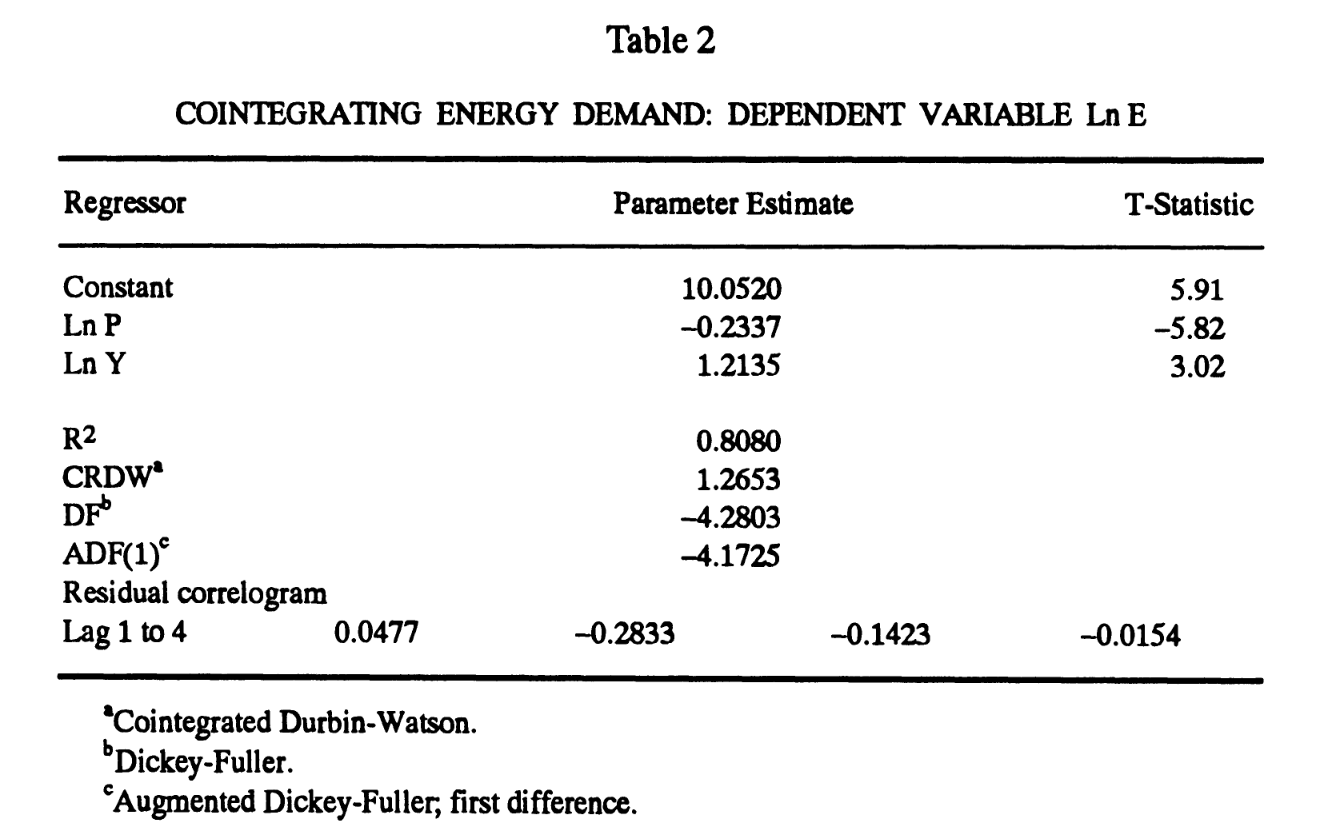
\includegraphics[width=0.8\textwidth]{./figure/ch1/fig1.1_table2.png}
	\caption{Cointegrating energy demand from \cref{eq1.2}. The parameter estimates for $\ln(P)$ and $\ln(Y)$ are the \textbf{long-run price- and income- elasticities}}\label{fig1.1}
\end{figure}

\begin{figure}[h]  % htbp
	\centering
	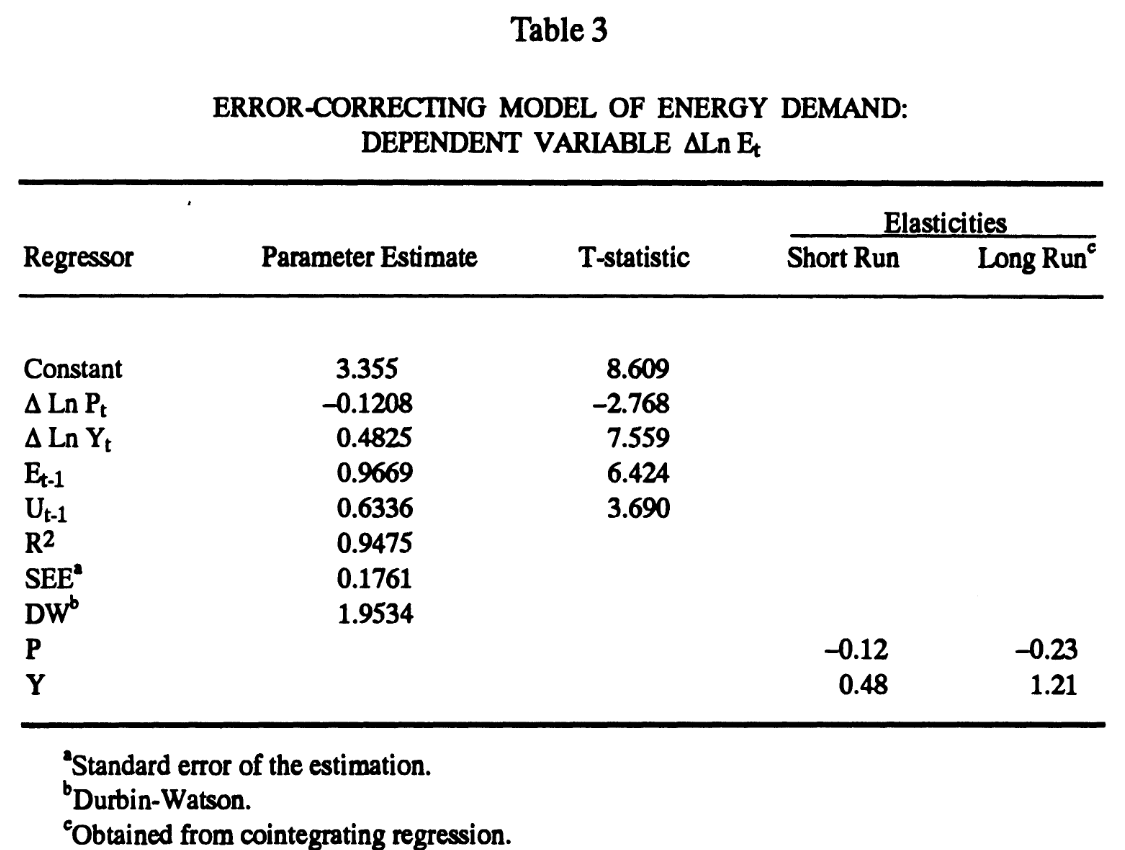
\includegraphics[width=0.8\textwidth]{./figure/ch1/fig1.2_table3.png}
	\caption{ECM of energy demand (\cref{eq1.3}). The parameter estimates for $\Delta \ln(P)$ and $\Delta \ln(Y)$ are the \textbf{short-run price- and income- elasticities}. }\label{fig1.2}
\end{figure}


%---- 1.1.2 Section 1.2 ----%
\subsection{Method 2: SEM}
	\paragraph{}{A \textbf{Simultaneous Equation Model (SEM)} assumed that the \textbf{desired} energy demand per capita ($E_t^*$) in year $t$ depends on the real price  of energy ($P_t$) and real per capita GDP ($Y_t$) in the form of a log-linear function. The planned energy demand could be written as
		\begin{equation}\label{eq1.5}
			\ln(E_t^*)=A_0 + A_1 \times \ln(P_t) + A_2 \times \ln(Y_t),
		\end{equation}}
	
	\paragraph{}{But the \textbf{actual} energy demand per capita ($E_t$) is not necessarily equal to the desired level due to technological rigidity and the inertia in endusers' decision making. The actual demand $E_t$ is thusly assumed to adjust towards the $E_t^*$ with a lag such that it is a function of the current year's economic variables and the energy consumption in the previous year ($t-1$), as indicated by \cref{eq1.6}.
		\begin{equation}\label{eq1.6}
			\ln(E_t)= \delta \times (A_0 + A_1 \times \ln(P_t) + A_2 \times \ln(Y_t)) + (1-\delta) \times \ln(E_{t-1}),
		\end{equation}
	where $\delta(\in [0,1])$ and $(1-\delta)$ are the weighting coefficient between the current economic variables and the inertia from the previous year.  $A_1$ and $A_2$ are the price- and income- elasticities. 
	}

	\paragraph{}{$Y_t$ is an endogenous variable which depends upon the level of energy consumption ($E_t$), whose output is altered by the technology and the structure of the economy. The structural and technological characteristics are measured by \textit{the percentage of output by the nonoil sectors $S_t$}. The relation is depicted as:
		\begin{equation}\label{eq1.7}
			\ln(Y_t) = C_0 + C_1 \times \ln(E_t) + C_2 \times \ln(S_t),
		\end{equation} \\
	\cref{eq1.6} and \cref{eq1.7} are simultaneously and endogenously determined using a two-stage least square method. 
	}

	\paragraph{Implementation\\}{The cointegration tests performed at the log level of the variables indicated nonstationarity but cointegration among the log-variables. The authors therefore used the undifferenced forms of the variables to preserve the information about long-run relationships. The statistical results of the SEM are shown in \cref{fig1.3}.}
	
	\begin{figure}[h]  % htbp
		\centering
		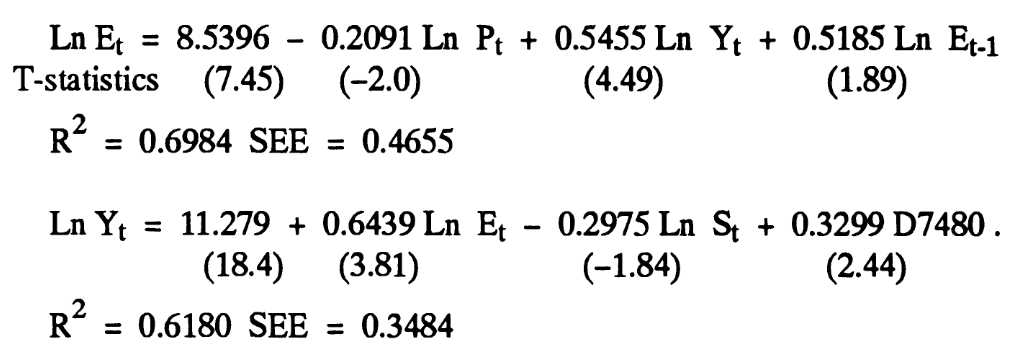
\includegraphics[width=0.8\textwidth]{./figure/ch1/fig1.3_result4.png}
		\caption{Statistical results of the SEM (\cref{eq1.6} and \cref{eq1.7}). The short-run price- and income- elasticities are -0.2091 and 0.5455 respectively. The long-run price elasticity = $-0.2091/(1-0.5185)=-0.4343$. The long-run income elasticity = $0.5455/(1-0.5185)=1.1329$.}\label{fig1.3}
	\end{figure}


%%---- Section 1.2 ----%
%\section{Discrete-continuous choice model}
%
%
%\section{Quantifier}
%\lipsum % dummy text - remove from real document
%
%\section{Graph}
%\citetitle{babaiGraphIsomorphismQuasipolynomial2016}
%\cite{babaiGraphIsomorphismQuasipolynomial2016}
%
%\section{Number theory}
%a Figure example
%\begin{figure}[!ht]
%    \centering
%    \includegraphics[width=1\linewidth]{./figure/elliptic_curves.pdf}
%    \caption{Elliptic curves \cite{childsUniversalComputationQuantum2009} }
%\end{figure}
%
%
%\section{Algorithm}
%% \begin{center}
%% \begin{minipage}{.9\linewidth}
%% algorithm2e
%% https://www.overleaf.com/learn/latex/Algorithms#The_algorithm2e_package
%\begin{algorithm}[H]
%    \DontPrintSemicolon
%    \SetKwInOut{Input}{input}
%    \SetKwInOut{Output}{output}
%    \Input{Integer $N$ and parameter $1^t$}
%    \Output{A decision as to whether $N$ is prime or composite}
%    \BlankLine
%    \For{ $i = 1,2, \ldots, t$} {
%        $a\leftarrow \qty{1,\dots,N_1}$  \tcp*{this is a comment}
%        \If{$a^{N-1} \neq 1 \mod{N}$}
%        % \tcc{comment in a new line}
%    {\Return "composite"}
%    }
%    \Return "prime"
%    \caption{Primality testing - first attempt}
%    \label{alg:miller_rabin}
%\end{algorithm}
%% \end{minipage}
%% \end{center}